% ID/OOD teaser figure for the rule-conditioned NCA WM paper.
%
% Single-document standalone TikZ figure.
%
% Per game row: a "card pair" — a code Box flush against the WEST
% (left, reading-order back) face of the PuzzleScript state Box. Both
% boxes are the same height and use a transparent fill so the
% projected face content (state image / code text) reads cleanly.
%
% Each NCA-WM block uses the same Encoder layout as nca_arch_v1.tex
% (2 self-attn + 1 cross-attn tflayer rectangles wrapped in a fit
% node). Code arrows from each row fan into the Encoder; the encoder
% output is connected by a dashed conditioning line up to a large
% latent-space PCA scatter sitting above the figure (train-only on
% the ID side; train + OOD stars on the eval side).
%
\documentclass[border=4pt, multi, tikz]{standalone}
\usepackage{amsmath}
\usepackage{amssymb}
\usepackage{import}
\subimport{../architecture/}{init}
\usetikzlibrary{positioning}
\usetikzlibrary{calc}
\usetikzlibrary{fit}
\usetikzlibrary{3d}
\usetikzlibrary{decorations.pathreplacing}

\colorlet{NCAColor}{green!35}
\colorlet{NCABandColor}{green!70}
\colorlet{EmbedColor}{green!12}
\colorlet{ReadoutColor}{red!18}
\colorlet{EncColor}{blue!18}
\colorlet{EncBandColor}{blue!50}
\colorlet{PSFrameFill}{gray!12}
\colorlet{CodeFill}{white}

\colorlet{IDColor}{blue!55!black}
\colorlet{OODColor}{red!55!black}
\colorlet{LossColor}{orange!85!black}
\colorlet{CondColor}{violet!60!black}

% Encoder rectangle style matches nca_arch_v1.tex but scaled down.
\tikzstyle{tflayer}=[draw, rounded corners=1.0pt, line width=0.3pt,
    minimum width=0.30cm, minimum height=1.10cm, inner sep=1pt]

% --- PS state frame, transparent so the image is the focus. ---
\newcommand{\PSframe}[4]{%
  \pic[shift={(#2, #3, 0)}] at (0,0,0)
      {Box={name=#1, caption=, xlabel={{,}}, zlabel={},
            fill=PSFrameFill, opacity=0.35,
            height=4, width=1.0, depth=4}};%
  \node[canvas is zy plane at x={#2 + 0.2}] at (0, #3)
      {\includegraphics[width=0.8cm,height=0.8cm]{#4}};%
}

% --- Card pair: transparent code Box flush LEFT of a transparent
%     state Box (reading-order "behind"). Same height/depth on both.
%     State image projected on state's east face; code text projected
%     on code's east face (= state's west, in the boundary plane).
%
%     Anchors: <name>g (state box), <name>c (code box).
%     #1 = name base, #2 = x_state, #3 = y, #4 = state image, #5 = code text
\newcommand{\StateOnCode}[5]{%
  \pic[shift={({#2 - 0.2}, #3, 0)}] at (0,0,0)
      {Box={name=#1c, caption=, xlabel={{,}}, zlabel={},
            fill=CodeFill, opacity=0.35,
            height=4, width=1.0, depth=4}};%
  % code text projected on code-box east face (the shared west of state)
  \node[canvas is zy plane at x={#2}, font=\tiny\ttfamily,
        align=left, inner sep=0pt, text width=0.78cm,
        anchor=center]
        at (0, #3) {#5};%
  \pic[shift={(#2, #3, 0)}] at (0,0,0)
      {Box={name=#1g, caption=, xlabel={{,}}, zlabel={},
            fill=PSFrameFill, opacity=0.35,
            height=4, width=1.0, depth=4}};%
  \node[canvas is zy plane at x={#2 + 0.2}] at (0, #3)
      {\includegraphics[width=0.8cm,height=0.8cm]{#4}};%
}

% --- NCA-WM block: nca_arch_v1.tex-style Encoder + Embed + 3 NCA bands
%     + Readout, plus a faint loop arrow under the body.
%     #1 = name suffix, #2 = x_center, #3 = y_center
\newcommand{\NCAblock}[3]{%
  % Encoder: 2 self-attn + 1 cross-attn (matches nca_arch_v1.tex).
  \node[tflayer, fill=EncColor] (encS1_#1)
      at ({#2 - 2.5}, #3) {};
  \node[tflayer, fill=EncColor, right=0.06cm of encS1_#1] (encS2_#1) {};
  \node[tflayer, fill=EncBandColor, right=0.06cm of encS2_#1] (encX_#1) {};
  \node[font=\tiny, rotate=90, inner sep=0pt] at (encS1_#1) {self-attn};
  \node[font=\tiny, rotate=90, inner sep=0pt] at (encS2_#1) {self-attn};
  \node[font=\tiny, rotate=90, inner sep=0pt, text=white!92!black]
      at (encX_#1) {$K$-q xattn};
  \node[draw, rounded corners=2pt, line width=0.45pt,
        fit=(encS1_#1)(encX_#1), inner sep=2pt] (enc_#1) {};
  % Embed
  \pic[shift={({#2 - 1.0}, #3, 0)}] at (0,0,0)
      {Box={name=embed_#1, caption=, xlabel={{,}}, zlabel={},
            fill=EmbedColor, height=8, width=1.5, depth=8}};
  % NCA bands
  \pic[shift={({#2 + 0.4}, #3, 0)}] at (0,0,0)
      {RightBandedBox={name=nca_#1, caption=, xlabel={{,,}}, zlabel={},
            fill=NCAColor, bandfill=NCABandColor,
            height=8, width={1.5,1.5,1.5}, depth=8}};
  % Readout
  \pic[shift={({#2 + 2.1}, #3, 0)}] at (0,0,0)
      {Box={name=readout_#1, caption=, xlabel={{,}}, zlabel={},
            fill=ReadoutColor, height=8, width=1.5, depth=8}};
  % Forward connections
  \draw[connection, -Stealth] (embed_#1-east) -- (nca_#1-west);
  \draw[connection, -Stealth] (nca_#1-east)   -- (readout_#1-west);
  % Encoder cross-attn output → NCA bands top (slot conditioning)
  \draw[condarrow] (encX_#1.east)
      to[out=10, in=120]
      ($(nca_#1-north)+(0,0)$);
  % Iteration loop arrow under the body
  \path let \p1 = (nca_#1-east), \p2 = (nca_#1-west) in
    coordinate (loopOutR_#1)  at (\x1+0.25cm, \y1)
    coordinate (loopOutRD_#1) at (\x1+0.25cm, \y1-1.0cm)
    coordinate (loopInLD_#1)  at (\x2-0.35cm, \y2-1.0cm)
    coordinate (loopInL_#1)   at (\x2-0.35cm, \y2);
  \draw[-Stealth, line width=0.4mm, opacity=0.32, rounded corners=4pt]
      (nca_#1-east) -- (loopOutR_#1) -- (loopOutRD_#1)
      -- (loopInLD_#1) -- (loopInL_#1) -- (nca_#1-west);
}

\begin{document}

\begin{tikzpicture}
\tikzstyle{connection}=[thick, every node/.style={sloped,allow upside down},
    draw=\edgecolor, opacity=0.7]
\tikzstyle{arrow}=[-Stealth, line width=0.3mm, opacity=0.85]
\tikzstyle{lossarrow}=[-Stealth, line width=0.3mm, color=LossColor]
\tikzstyle{condarrow}=[-Stealth, line width=0.3mm, dashed,
    color=CondColor, opacity=0.9]
\tikzstyle{condline}=[line width=0.35mm, dashed,
    color=CondColor, opacity=0.85]
\tikzstyle{ardashed}=[-Stealth, line width=0.25mm, dashed,
    color=OODColor, opacity=0.9]

% =============================================================
%  LEFT HALF: in-distribution training (NCA-WM at x=-3)
% =============================================================
\NCAblock{id}{-3}{0}

\StateOnCode{neko}{-7}{ 1.5}{rollouts/nekopuzzle/engine_t0.png}
    {;nekopuzzle\\{}[>P|...|F]\\->[|...|P]}
\StateOnCode{soko}{-7}{ 0.0}{rollouts/sokoban_basic/engine_t0.png}
    {;sokoban\\{}[>P|C]\\->[>P|>C]}
\StateOnCode{mod} {-7}{-1.5}{rollouts/Modality/engine_t0.png}
    {;modality\\{}[>PW|B]\\->CANCEL}

\PSframe{s1_neko}{1.0}{ 1.5}{rollouts/nekopuzzle/engine_t1.png}
\PSframe{s1_soko}{1.0}{ 0.0}{rollouts/sokoban_basic/engine_t1.png}
\PSframe{s1_mod} {1.0}{-1.5}{rollouts/Modality/engine_t1.png}

% Latent-space inset ABOVE the ID encoder, large
\node[anchor=south, inner sep=1pt] (latent_id) at (-5.6, 3.0)
    {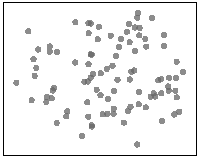
\includegraphics[width=2.6cm]{latent_train_only.pdf}};
\node[font=\tiny\itshape, color=IDColor, anchor=south]
    at (-5.6, 5.55) {encoder latent space};
% Dashed line: encoder top → latent scatter bottom
\draw[condline] (enc_id.north) -- (latent_id.south);

% State (blue) fan-in from each game's state box to embed
\draw[arrow, color=IDColor] (nekog-east) -- (embed_id-west);
\draw[arrow, color=IDColor] (sokog-east) -- (embed_id-west);
\draw[arrow, color=IDColor] (modg-east)  -- (embed_id-west);

% Code (dashed violet) fan-in to encoder
\draw[condarrow] (nekoc-east) to[out=15,in=160] (enc_id.west);
\draw[condarrow] (sokoc-east) to[out=10,in=170] (enc_id.west);
\draw[condarrow] (modc-east)  to[out=-15,in=200] (enc_id.west);

% Loss (dark orange) fan-in to readout
\draw[lossarrow] (s1_neko-west) -- (readout_id-east);
\draw[lossarrow] (s1_soko-west) -- (readout_id-east);
\draw[lossarrow] (s1_mod-west)  -- (readout_id-east);

% ID banner
\node[font=\footnotesize\bfseries, color=IDColor, anchor=south, align=center]
    at (-3, 5.95) {Training (in-distribution)};

% =============================================================
%  VERTICAL DASHED BORDER between train and eval
% =============================================================
\draw[dashed, line width=0.3mm, color=black!70]
    (2.5, -2.4) -- (2.5,  6.2);
\node[font=\itshape\tiny, color=black!50, anchor=south, rotate=90]
    at (2.75, 0.4) {trained $\theta \rightarrow \theta^{*}$};

% =============================================================
%  RIGHT HALF: held-out eval (NCA-WM at x=+7)
% =============================================================
\NCAblock{ood}{7}{0}

\StateOnCode{inway}{ 3.5}{ 1.5}
    {rollouts/in_the_way_by_giovanni_mota/pred_t0.png}
    {;in\_the\_way\\{}[>P|F]\\->[|P]}
\StateOnCode{nana}{ 3.5}{ 0.0}
    {rollouts/my_nana_ate_my_kid_brother_by_ruth_williams/pred_t0.png}
    {;my\_nana\\late[G|.|P]\\->[T|.|G]}
\StateOnCode{ham}{ 3.5}{-1.5}
    {rollouts/Hamiltwo/pred_t0.png}
    {;hamiltwo\\{}[>L|noW]\\->[>L+|noW]}

\PSframe{h1_inway}{10.5}{ 1.5}{rollouts/in_the_way_by_giovanni_mota/pred_t1.png}
\PSframe{h2_inway}{11.7}{ 1.5}{rollouts/in_the_way_by_giovanni_mota/pred_t2.png}
\PSframe{h3_inway}{12.9}{ 1.5}{rollouts/in_the_way_by_giovanni_mota/pred_t3.png}

\PSframe{h1_nana}{10.5}{ 0.0}{rollouts/my_nana_ate_my_kid_brother_by_ruth_williams/pred_t1.png}
\PSframe{h2_nana}{11.7}{ 0.0}{rollouts/my_nana_ate_my_kid_brother_by_ruth_williams/pred_t2.png}
\PSframe{h3_nana}{12.9}{ 0.0}{rollouts/my_nana_ate_my_kid_brother_by_ruth_williams/pred_t3.png}

\PSframe{h1_ham}{10.5}{-1.5}{rollouts/Hamiltwo/pred_t1.png}
\PSframe{h2_ham}{11.7}{-1.5}{rollouts/Hamiltwo/pred_t2.png}
\PSframe{h3_ham}{12.9}{-1.5}{rollouts/Hamiltwo/pred_t3.png}

% Latent-space inset ABOVE the OOD encoder, large
\node[anchor=south, inner sep=1pt] (latent_ood) at (4.4, 3.0)
    {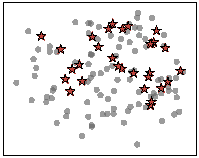
\includegraphics[width=2.6cm]{latent_with_ood.pdf}};
\node[font=\tiny\itshape, color=OODColor, anchor=south]
    at (4.4, 5.55) {encoder latent space + OOD ($\bigstar$)};
\draw[condline] (enc_ood.north) -- (latent_ood.south);

% State fan-in
\draw[arrow, color=OODColor] (inwayg-east) -- (embed_ood-west);
\draw[arrow, color=OODColor] (nanag-east)  -- (embed_ood-west);
\draw[arrow, color=OODColor] (hamg-east)   -- (embed_ood-west);

% Code fan-in to encoder
\draw[condarrow] (inwayc-east) to[out=15,in=160] (enc_ood.west);
\draw[condarrow] (nanac-east)  to[out=10,in=170] (enc_ood.west);
\draw[condarrow] (hamc-east)   to[out=-15,in=200] (enc_ood.west);

% ŝ_1 fan-out
\draw[arrow, color=OODColor] (readout_ood-east) -- (h1_inway-west);
\draw[arrow, color=OODColor] (readout_ood-east) -- (h1_nana-west);
\draw[arrow, color=OODColor] (readout_ood-east) -- (h1_ham-west);

% Autoregressive dashed chain
\draw[ardashed] (h1_inway-east) -- (h2_inway-west);
\draw[ardashed] (h2_inway-east) -- (h3_inway-west);
\draw[ardashed] (h1_nana-east)  -- (h2_nana-west);
\draw[ardashed] (h2_nana-east)  -- (h3_nana-west);
\draw[ardashed] (h1_ham-east)   -- (h2_ham-west);
\draw[ardashed] (h2_ham-east)   -- (h3_ham-west);

% OOD banner
\node[font=\footnotesize\bfseries, color=OODColor, anchor=south, align=center]
    at (8, 5.95) {Evaluation (held-out / OOD)};

\node[font=\itshape\tiny, color=OODColor, anchor=north, align=center]
    at (11.7, -1.95)
    {$\hat s_{t+1}$ fed back (autoregressive); no supervision};

\end{tikzpicture}

\end{document}
